% SPDX-License-Identifier: BSD-2-Clause
%
% Copyright (C) 2026 embedded brains GmbH & Co. KG
%
% Redistribution and use in source and binary forms, with or without
% modification, are permitted provided that the following conditions
% are met:
% 1. Redistributions of source code must retain the above copyright
%    notice, this list of conditions and the following disclaimer.
% 2. Redistributions in binary form must reproduce the above copyright
%    notice, this list of conditions and the following disclaimer in the
%    documentation and/or other materials provided with the distribution.
%
% THIS SOFTWARE IS PROVIDED BY THE COPYRIGHT HOLDERS AND CONTRIBUTORS "AS IS"
% AND ANY EXPRESS OR IMPLIED WARRANTIES, INCLUDING, BUT NOT LIMITED TO, THE
% IMPLIED WARRANTIES OF MERCHANTABILITY AND FITNESS FOR A PARTICULAR PURPOSE
% ARE DISCLAIMED. IN NO EVENT SHALL THE COPYRIGHT OWNER OR CONTRIBUTORS BE
% LIABLE FOR ANY DIRECT, INDIRECT, INCIDENTAL, SPECIAL, EXEMPLARY, OR
% CONSEQUENTIAL DAMAGES (INCLUDING, BUT NOT LIMITED TO, PROCUREMENT OF
% SUBSTITUTE GOODS OR SERVICES; LOSS OF USE, DATA, OR PROFITS; OR BUSINESS
% INTERRUPTION) HOWEVER CAUSED AND ON ANY THEORY OF LIABILITY, WHETHER IN
% CONTRACT, STRICT LIABILITY, OR TORT (INCLUDING NEGLIGENCE OR OTHERWISE)
% ARISING IN ANY WAY OUT OF THE USE OF THIS SOFTWARE, EVEN IF ADVISED OF THE
% POSSIBILITY OF SUCH DAMAGE.

\documentclass[tikz,border=4pt]{standalone}
\usepackage[T1]{fontenc}
\usepackage[scaled]{helvet}
\renewcommand{\familydefault}{\sfdefault}
\usetikzlibrary{arrows.meta,positioning,fit,backgrounds,shapes.geometric}
\definecolor{ebblue}{HTML}{1F4E79}
\definecolor{boxfill}{HTML}{EAF1F8}
\definecolor{codefill}{HTML}{FFF4E0}
\definecolor{codeline}{HTML}{9C6500}
\definecolor{groupfill}{HTML}{F5F5F5}
\definecolor{flow}{HTML}{404040}
\newcommand{\code}[1]{{\ttfamily\scriptsize #1}}
\begin{document}
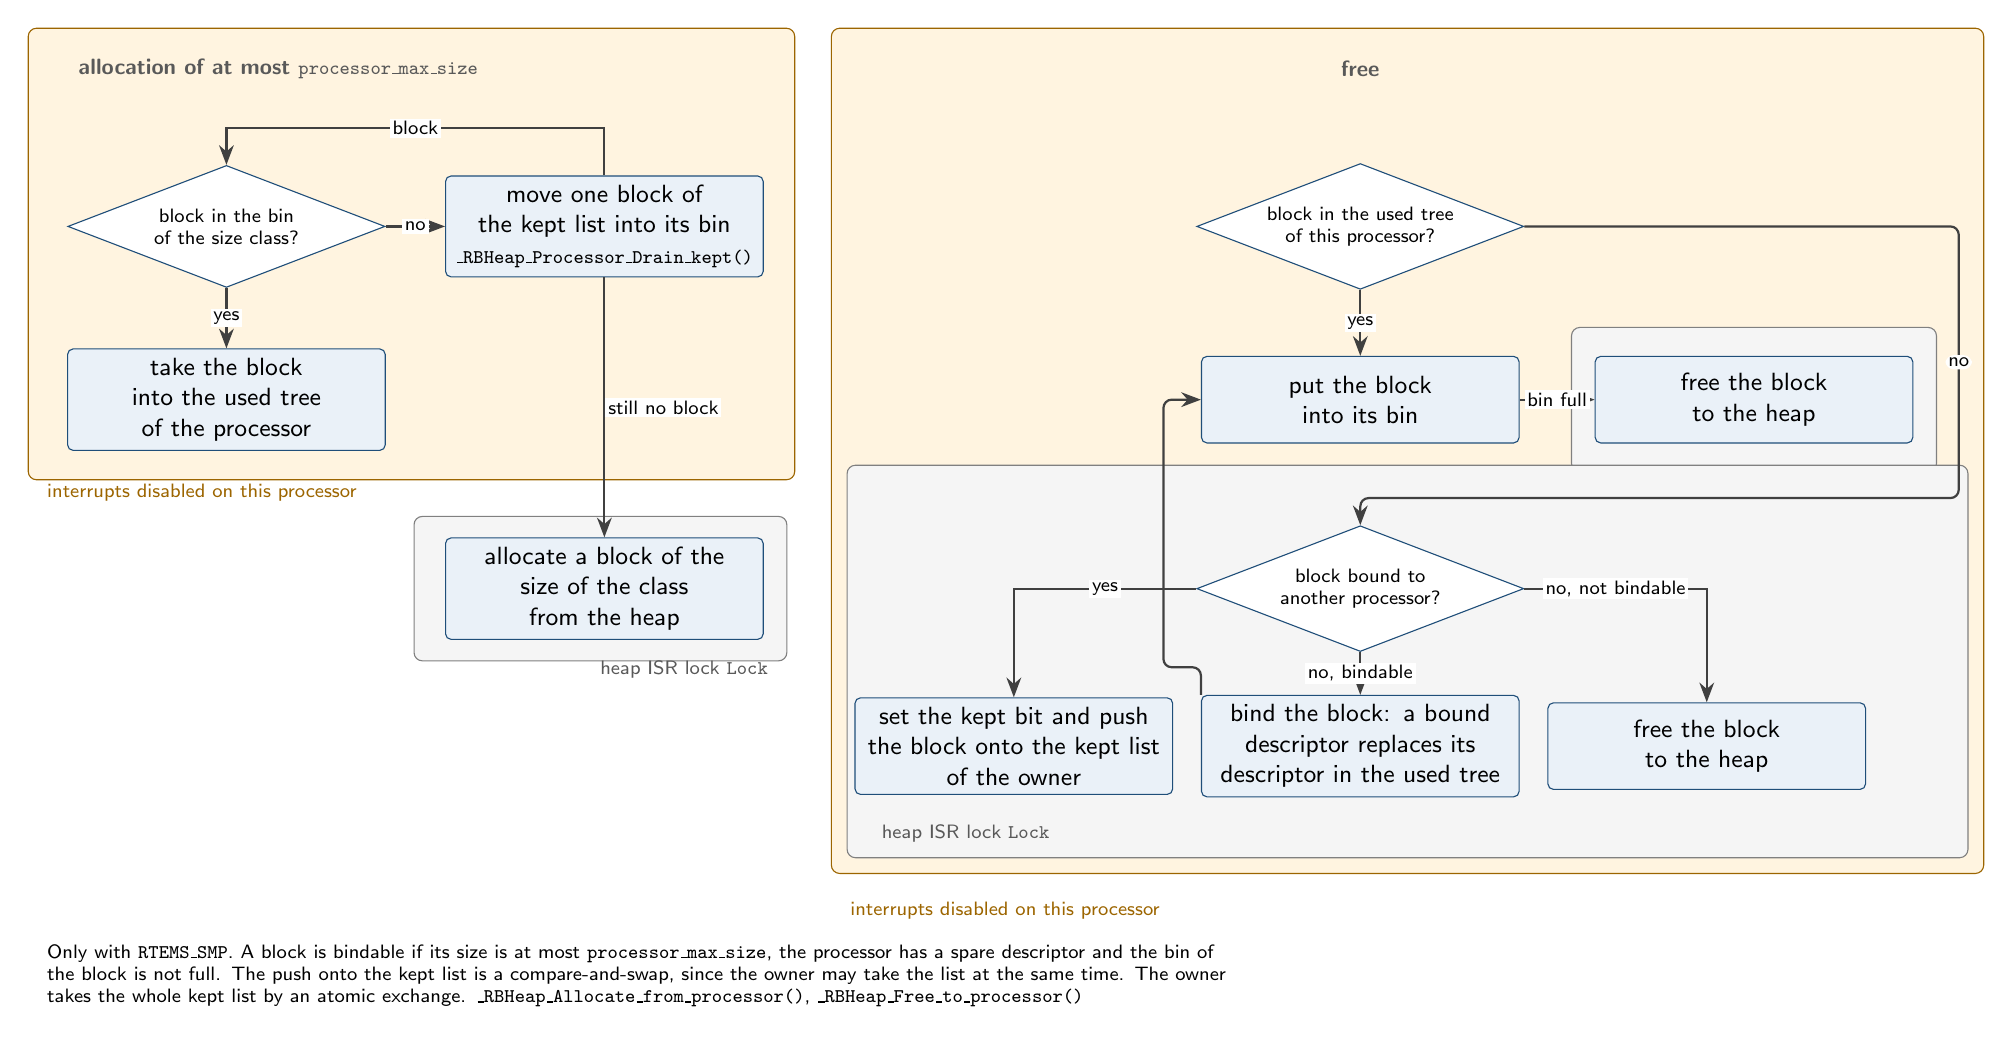
\begin{tikzpicture}[
    font=\small,
    act/.style={draw=ebblue, fill=boxfill, rounded corners=2pt,
      minimum width=40mm, minimum height=11mm, align=center, text width=38mm},
    dec/.style={draw=ebblue, fill=white, diamond, aspect=2.6, inner sep=1pt,
      align=center, font=\scriptsize, text width=26mm},
    trans/.style={-{Stealth[length=2.5mm]}, thick, draw=flow},
    yes/.style={font=\scriptsize, fill=white, inner sep=1pt},
    irqframe/.style={fill=codefill, draw=codeline, rounded corners=3pt},
    lockframe/.style={fill=groupfill, draw=gray, rounded corners=3pt},
    title/.style={font=\footnotesize\bfseries, text=gray!70!black}]
  % Allocation
  \node[title, anchor=west] at (0,2.0) {allocation of at most \code{processor\_max\_size}};
  \node[dec] (hit) at (2.0,0) {block in the bin\\of the size class?};
  \node[act] (take) at (2.0,-2.2) {take the block\\into the used tree\\of the processor};
  \node[act] (kept) at (6.8,0) {move one block of\\the kept list into its bin\\\code{\_RBHeap\_Processor\_Drain\_kept()}};
  \node[act] (heap) at (6.8,-4.6) {allocate a block of the\\size of the class\\from the heap};
  \draw[trans] (hit) -- node[yes] {yes} (take);
  \draw[trans] (hit) -- node[yes] {no} (kept);
  \draw[trans] (kept) -- node[yes, right] {still no block} (heap);
  \draw[trans] (kept.north) |- ++(0,0.6) -| node[yes, pos=0.25] {block} (hit.north);
  % Free
  \node[title] at (16.4,2.0) {free};
  \node[dec] (own) at (16.4,0) {block in the used tree\\of this processor?};
  \node[act] (bin) at (16.4,-2.2) {put the block\\into its bin};
  \node[act] (full) at (21.4,-2.2) {free the block\\to the heap};
  \node[dec] (bound) at (16.4,-4.6) {block bound to\\another processor?};
  \node[act] (push) at (12.0,-6.6) {set the kept bit and push\\the block onto the kept list\\of the owner};
  \node[act] (bind) at (16.4,-6.6) {bind the block: a bound\\descriptor replaces its\\descriptor in the used tree};
  \node[act] (free) at (20.8,-6.6) {free the block\\to the heap};
  \draw[trans] (own) -- node[yes] {yes} (bin);
  \draw[trans] (bin) -- node[yes] {bin full} (full);
  \draw[trans, rounded corners=3pt] (own.east) -- (24.0,0) |- node[yes, pos=0.25] {no} (16.4,-3.45) -- (bound.north);
  \draw[trans] (bound) -| node[yes, pos=0.25] {yes} (push);
  \draw[trans] (bound) -- node[yes] {no, bindable} (bind);
  \draw[trans] (bound) -| node[yes, pos=0.25] {no, not bindable} (free);
  \draw[trans, rounded corners=3pt] (bind.north west) -- ++(0,0.35) -| (13.9,-2.2) -- (bin.west);
  % Lock scopes
  \begin{scope}[on background layer]
    \node[irqframe, fit={(-0.4,2.4) (9.1,-3.1)}] {};
    \node[irqframe, fit={(9.8,2.4) (24.2,-8.1)}] {};
    \node[lockframe, fit={(4.5,-3.8) (9.0,-5.4)}] {};
    \node[lockframe, fit={(19.2,-1.4) (23.6,-3.0)}] {};
    \node[lockframe, fit={(10.0,-3.15) (24.0,-7.9)}] {};
  \end{scope}
  \node[font=\scriptsize, text=codeline, anchor=north west] at (-0.4,-3.15) {interrupts disabled on this processor};
  \node[font=\scriptsize, text=gray!70!black, anchor=south west] at (10.2,-7.95) {heap ISR lock \code{Lock}};
  \node[font=\scriptsize, text=gray!70!black, anchor=north east] at (9.0,-5.4) {heap ISR lock \code{Lock}};
  \node[font=\scriptsize, text=codeline, anchor=north west] at (9.8,-8.45) {interrupts disabled on this processor};
  \node[font=\scriptsize, anchor=north west, text width=150mm] at (-0.4,-9.0)
    {Only with \code{RTEMS\_SMP}.  A block is bindable if its size is at most
     \code{processor\_max\_size}, the processor has a spare descriptor and the bin
     of the block is not full.  The push onto the kept list is a
     compare-and-swap, since the owner may take the list at the same time.  The
     owner takes the whole kept list by an atomic exchange.
     \code{\_RBHeap\_Allocate\_from\_processor()},
     \code{\_RBHeap\_Free\_to\_processor()}};
\end{tikzpicture}
\end{document}
